\documentclass[12pt, letterpaper]{umthesis}

%%%%%%%%%%%%%%%%%%%%%%%%%%%%%%%%%%%%%%%%%%%%%%%%%%%%%%%%%%%
%%%                  optional packages                  %%%
%%%%%%%%%%%%%%%%%%%%%%%%%%%%%%%%%%%%%%%%%%%%%%%%%%%%%%%%%%%
%% these packages are all optional. I include them here
%% because I use them, and I know they work with this class

\usepackage{sidecap} %put captions beside a figure
\usepackage{ifpdf} % check to see if compiling as dvi or pdf
\usepackage{rotating} % rotate some text
\usepackage{graphicx} % include graphics files
%\usepackage[all]{xy} %for making simple graphs
\usepackage{index} %this is newer and more fully featured than makeidx
\usepackage{hhline} %fancy rules
\usepackage{amsmath,amssymb} %extra math commands and symbols
\usepackage{mathptmx} %use times for normal text and math
\usepackage{helvet} %use helvetica font for sans-serif
\usepackage{courier} % use courier font for typewriter and fixed width
\usepackage{colortbl} %allows for color in tables
\usepackage{subfigure} % groups figures into one large one
\usepackage{longtable} % multi-page tables 
\usepackage{pdflscape} %better handling of landscape features
\usepackage{tabularx} %advanced tabular environment
\usepackage{multicol} % to use multiple columns
\usepackage{tikz} % package for making cool graphics - compatible with 
                  %  dvi, postscript, and pdf
\usetikzlibrary{arrows} % fancy arrows for tikz package
\usepackage{natbib} %more advanced handling of bibliographies
\bibpunct{(}{)}{;}{a}{,}{,} %settings for natbib, if using it
\usepackage[font=small,labelfont=bf,labelsep=quad]{caption} %more caption
\ifpdf %use these packages if we are compiling with pdf
  \usepackage{epstopdf} %automatically converts .eps files to .pdf
  \usepackage[final,expansion=true,protrusion=true]{microtype} 
    %advanced typesetting
\fi
%\usepackage[T1]{tipa} %phonetic fonts
%\usepackage{placeins} %prevent floats from floating past section
%\usepackage{flafter} %don't allow floats to appear before their definition
  %formatting
%\usepackage{chngpage}%this allows resetting margins within the document
%\usepackage[color]{showkeys}  % prints the names of labels that you use
                                 % handy for proofreading purposes
%\usepackage[dvips]{geometry} %tells dvips about paper size options
%\usepackage{svn} % to keep track of revisions
%\SVN $Author: robfelty $
%\SVN $Revision: 24 $
%\SVN $Date: 2007-05-10 15:13:37 -0400 (Thu, 10 May 2007) $
%\SVN $Id: example.tex 24 2007-05-10 19:13:37Z robfelty $
%\usepackage{timestamp} % to give me a timestamp

%%%%%%%%%%%%%%%%%%%%%%%%%%%%%%%%%%%%%%%%%%%%%%%%%%%%
%% sectsty allows to do some fancier formatting
%% of chapter and section titles - it is not clear
%% to me whether Rackham allows this or not
%%%%%%%%%%%%%%%%%%%%%%%%%%%%%%%%%%%%%%%%%%%%%%%%%%%

%\usepackage{sectsty}
%\makeatletter
%\chapternumberfont{%
%  \if@mainmatter%
%    \rule{\textwidth}{2pt}\\%
%    \vspace{-1em}\rule{\textwidth}{1pt}\\%
%  \fi%
%  \centering \huge \bf%
%}
%\chaptertitlefont{%
%  \if@mainmatter%
%    \vspace{-1em} \rule{\textwidth}{1pt}\\[.2em]%
%  \fi%
%  \centering \huge \bf%
%}
%\makeatother
%\usepackage[pdftex]{graphicx}

%%%%%%%%%%%%%%%%%%%%%%%%%%%%%%%%%%%%%%%%%%%%%%%%%%%%%%%%%%%
%%% fancy headers are not allowed by Rackham - however
%%% this does not mean that you can't use them for all other
%%% copies that you do not give to Rackham
%%%%%%%%%%%%%%%%%%%%%%%%%%%%%%%%%%%%%%%%%%%%%%%%%%%%%%%%%%%

%\usepackage{fancyhdr} 
%      \pagestyle{fancy} 
%      % with this we ensure that the chapter and section 
%      % headings are in lowercase. 
%      \renewcommand{\chaptermark}[1]{\markboth{#1}{}} 
%      \renewcommand{\sectionmark}[1]{\markright{\thesection\ #1}} 
%      \fancyhf{} % delete current setting for header and footer 
%      \fancyhead[LE,RO]{\thepage} 
%      \fancyhead[LO]{\rightmark} 
%      \fancyhead[RE]{\leftmark} 
%      %\fancyhead[RE,RO]{\bfseries\rightmark} 
%      %\fancyhead[LE,LO]{\bfseries\leftmark} 
%      %\fancyfoot[C]{\thepage}
%      \renewcommand{\headrulewidth}{0.5pt} 
%      \renewcommand{\footrulewidth}{0pt} 
%      \addtolength{\headheight}{0.5pt} % make space for the rule 
%      \fancypagestyle{plain}{% 
%      \fancyhead{} % get rid of headers on plain pages 
%      %\fancyfoot[C]{\thepage}
%      \fancyfoot{}
%      \renewcommand{\headrulewidth}{0pt} % and the line 
%      } 
\hfuzz2pt % Don't bother to report overfull hboxes if over-edge is < 2pt
\vfuzz2pt % Same for overfull vboxes (maybe just works for hfuzz?)  

%this command can be used for table headers that need to be rotated, thus the
%name rotth, for rotated table header -- it takes two arguments, the width of
%the parbox to create (which since it is rotated is more like height), and the
%text to put in it
\newcommand\rotth[2]{%
  \begin{sideways}%
    \parbox[b]{#1}{\raggedright #2}%
  \end{sideways}%
}
%this sets up a new command \dash, which makes nice dashes
\DeclareRobustCommand\dash{% 
\unskip\nobreak\thinspace\textemdash\thinspace\ignorespaces} 
   %in bookmarks, use regular dash instead of emdash
  \pdfstringdefDisableCommands{\renewcommand{\dash}{ - }} 

%%%%%%%%%%%%%%%%%%%%%%%%%%%%%%%%%%%%%%%%%%%%%%%%%%%%
%% additional options for the hyperref package (it is already loaded)
%%%%%%%%%%%%%%%%%%%%%%%%%%%%%%%%%%%%%%%%%%%%%%%%%%%%
%  \hypersetup{
%  colorlinks,
%  bookmarksnumbered,
%  bookmarkstype={toc},
%  bookmarksopen={true},
%  bookmarksopenlevel={1},
%  pdfstartview={FitH},
%  citecolor={blue},
%  %linkcolor={black},
%  %urlcolor={black},
%  pdfpagemode={UseOutlines},
%  breaklinks=true
%  } 

%the next two lines will prevent hyphenation in phonetic transcriptions
%\usepackage{hyphenat}
%\newcommand{\ipa}[1]{\nohyphens{\textipa{#1}}}

%% redefine some rules for nice table formatting
\setlength{\arrayrulewidth}{.6pt}
\setlength{\doublerulesep}{0pt}

%% allow more floats on a page, and change the float separation from text
\setlength{\floatsep}{5pt}
\setlength{\intextsep}{5pt}
\renewcommand\floatpagefraction{.70}
\renewcommand\topfraction{.95}
\renewcommand\bottomfraction{.95}
\renewcommand\textfraction{.1}

%%%%%%%%%%%%%%%%%%%%%%%%%%%%%%%%%%%%%%%%%%%%%%%%%%%%%%%%%%%
%%                    line spacing                      %%%
%% Rackham requires onehalf or double spacing
%% The default for the class is onehalf
%% To change it for non-final copies, use one of the following options
%\singlespacing
%\doublespacing
%% The class file automatically singles spaces stuff which should
%% be single spaced according to rackham, like the bibliography,
%% titles, long quotations and such
%% However, if you want to, you can also change spacing for 
%% a portion of text like so:
%%\begin{singlespacing} ... \end{singlespacing}
%%%%%%%%%%%%%%%%%%%%%%%%%%%%%%%%%%%%%%%%%%%%%%%%%%%%%%%%%%%

%%%%%%%%%%%%%%%%%%%%%%%%%%%%%%%%%%%%%%%%%%%%%%%%%%%%%%%%%%%
%%%               title and author info                %%%%
%%%%%%%%%%%%%%%%%%%%%%%%%%%%%%%%%%%%%%%%%%%%%%%%%%%%%%%%%%%
\author{\LaTeX}
\program{Professional Typesetting}
\degree{Doctor of Philosophy}
% if you only have chair, use \chaircommitteemember
% if you have outside members, you can specify their institution in the
% optional argument 
\cochaircommitteemember{John Smith}{Professor}
\cochaircommitteemember{Mary Johnson}{Assistant Professor}
\committeemember[University of Hard Knocks]{Robert Hughes}{Professor}
\committeemember{Emily Dickens}{Assistant Professor}
\title{The most Rackham-standards compliant dissertation ever}

\makeindex %if you are including an index
%%%%%%%%%%%%%%%%%%%%%%%%%%%%%%%%%%%%%%%%%%%%%%%%%%%%%%%%%%%%%%%%%
%% IMPORTANT - learn to use includeonly - it is very helpful
%% 1. put each chapter in a separate file
%% 2. type \include{file} where you want it to go
%% 3. First you have to compile once with everything included, 
%%    then you can include only certain parts
%%
%% and the table of contents will still list all parts, 
%% the chapter numbers will still all be correct
%% and you can easily print out (or e-mail or whatever) just one chapter
%% if you like, you can even leave out all the frontmatter stuff by putting
%% it in a separate file as well
%%%%%%%%%%%%%%%%%%%%%%%%%%%%%%%%%%%%%%%%%%%%%%%%%%%%%%%%%%%%%%%%%
\includeonly{%
intro,%
exp1,%
exp2,%
exp3,%
conclusion,%
appendix
}
\begin{document}
%%%%%%%%%%%%%%%%%%%%%%%%%%%%%%%%%%%%%%%%%%%%%%%%%%%%%%%%%%%%%%%%%%%%
%% IMPORTANT -- must issue frontmatter, mainmatter, and backmatter
%% commands in right place. These commands handle page numbering and
%%  formatting of various parts
%% \frontmatter - right after begin document
%% \mainmatter - right before first chapter
%% \backmatter - right before bibliography
%%%%%%%%%%%%%%%%%%%%%%%%%%%%%%%%%%%%%%%%%%%%%%%%%%%%%%%%%%%%%%%%%%%%%
\frontmatter

%%%% these command change latex's default hyphenation a bit. 
% Setting tolerance low will encourage hyphenation. 
% Setting tolerance high will discourage hyphenation
\pretolerance=-1
\tolerance=1000
\adjdemerits=6400
\doublehyphendemerits=90000
\finalhyphendemerits=14400

\maketitle
%%%%% the finalabstract environment typesets the abstract as it should be
% for the copies that go to Rackham separate of the actual dissertation. 
\begin{finalabstract}
  your abstract here
\end{finalabstract}
\makecopyright

\begin{frontispiece}
  If we knew what we were doing, it wouldn't be called research\\
  \dash Albert Einstein
\end{frontispiece}

\begin{dedication}
  to Delores
\end{dedication}

\begin{acknowledgments}
  these people helped me
\end{acknowledgments}

\begin{preface}
  before reading this, you should know\dots
\end{preface}

\tableofcontents

% only use these commands if you have more than figure, table, and/or
% appendix, respectively
\listoftables
\listoffigures
\listofappendices

% the normal abstract is formatted the same as preface and acknowledgments,
% and is listed in the table of contents
\begin{abstract}
  your abstract here
\end{abstract}
\mainmatter
\section{Introduction}
\label{sec:introduction}

To accompany \TeX{}, Knuth developed \MF{} as a method of ``creating
entire families of fonts from a set of dimensional parameters and
outline descriptions''~\cite{beebe:mf}.  Approximately ten years later,
John Hobby began work on \MP{}\Dash ``a powerful graphics language based
on Knuth's \MF, but with PostScript output and facilities for including
typeset text''~\cite{hobby:user}.  Although several packages (e.g.,
\PiC\TeX, \Xy-pic, and the native \LaTeX{} picture environment to name a
few) are available for creating graphics within \TeX-based documents,
they all rely on \TeX{}.  Since \TeX{} was designed to typeset text, it
seems natural that an external utility should be used to generate
graphics instead.  Furthermore, in the event that the graphics require
typeset text, then the utility should use \TeX{} for this requirement.
This premise is exactly the philosophy of \MP.

Since \MP{} is a programming language, it accommodates data structures
and flow control, and compilation of the \MP{} source code yields \EPS{}
graphics.  These features provide an elegant method for generating
graphics.  \autoref{fig:circles} illustrates how \MP{} can be used
programatically.  The figure is generated by rotating one of the circles
multiple times to obtain the desired \textit{circular chain}.%
\footnote{All graphics in this tutorial (except \autoref{fig:previewer})
  are created with \MP{}, and the source code and any required external
  data files for each of these graphics are embedded as file attachments
  in the electronic \PDF{} version of the article.  Attachments are
  indicated by a paper clip icon.

  \vspace{-\baselineskip}
  \noindent%
  \raisebox{0pt}[0pt][0pt]{%
    \makebox[0pt][r]{%
      \notextattachfile{\paperclip}%
      \hspace*{\marginparsep}%
    }%
  }%
}

\begin{figure}
  \begin{withattachment}{circles.mp}
    \centering
    \includegraphics{circles.mps}
  \end{withattachment}
  \caption{Rotated circles}
  \label{fig:circles}
\end{figure}

The programming language constructs of \MP{} also deliver a graceful
mechanism for creating animations without having to manually create each
frame of the animation.  The primary advantage of \EPS{} is that it can
be scaled to any resolution without a loss in quality.  It can also be
easily converted to raster formats, e.g.\ Portable Network Graphics
(\PNG) and Joint Photographic Experts Group (\JPEG), et al., or other
vector formats including Portable Document Format (\PDF) and Scalable
Vector Graphics (\SVG), et al.

\chapter{My first experiment}
\label{ch:firstExp}

This is my first experiment. I will try to prove the following things:
(Note that lists are single spaced, as Rackham wants, and that lists should
start a new paragraph, otherwise the single spacing will also apply to the
preceding paragraph).

\begin{itemize}
  \item lists are easy to use
  \item \LaTeX\ rocks
\end{itemize}

The following figure was drawn using the excellent pgf/tikz graphics package.
If you do not have this package, you should comment it out.

\begin{figure*}[htbp]
\centering
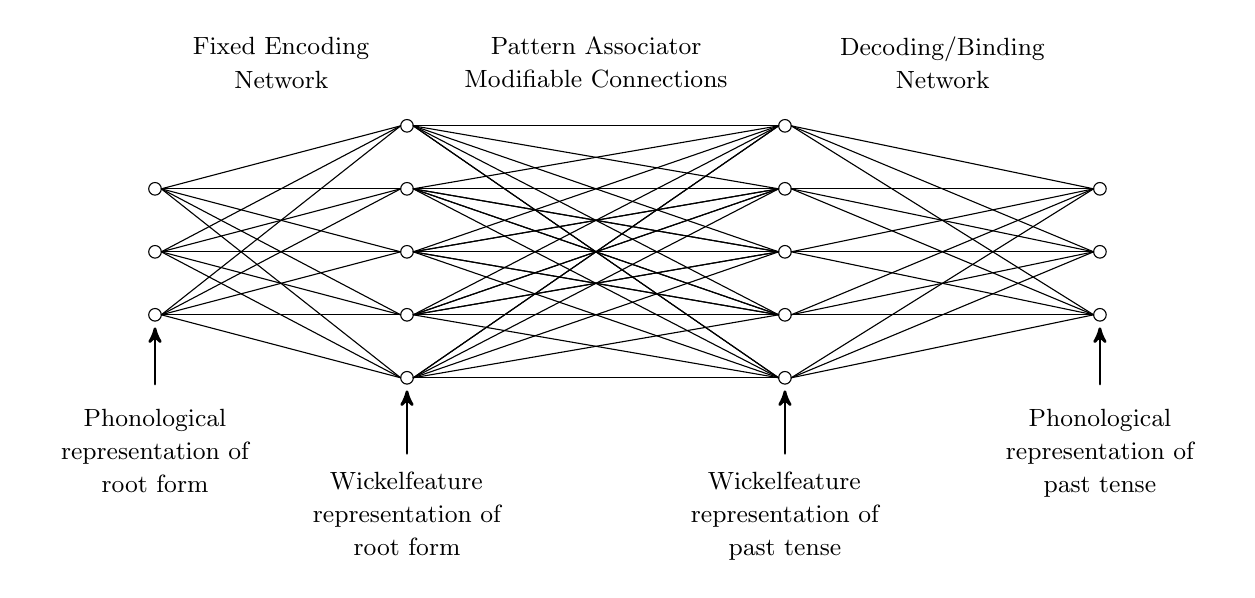
\begin{tikzpicture}[scale=.8,cap=round] 
% Styles 
\tikzstyle{information text}=[text badly centered]%, rounded corners,fill=red!10,inner sep=1ex] 
% The graphic 
\begin{scope}
\pgfsetarrowsend{stealth'} 
\pgfsetlinewidth{1pt} 
\draw (1,.9) -- (1,1.8)
  node[below=.9cm,text width=3cm,style=information text] 
  {\small Phonological representation of root form }; 
\draw (5,-.2) -- (5,.8)
  node[below=.9cm,text width=3cm, style=information text] 
  { \small Wickelfeature representation of root form }; 
\draw (11,-.2) -- (11,.8)
  node[below=.9cm,text width=3cm, style=information text] 
  { \small Wickelfeature representation of past tense }; 
\draw (16,0.9) -- (16,1.8)
  node[below=.9cm,text width=3cm, style=information text] 
  { \small Phonological representation of past tense }; 
\end{scope}
\draw (3,6)
  node[text width=3cm, style=information text] 
  { \small Fixed Encoding Network };
\draw (8,6)
  node[text width=4cm, style=information text] 
  { \small Pattern Associator Modifiable Connections };
\draw (13.5,6)
  node[text width=3cm, style=information text] 
  { \small Decoding/Binding Network };
% draw the nodes
\foreach \x in {1,16} 
  \foreach \y in {2,3,4} { 
    \draw (\x,\y) circle (0.1cm); 
  } 
\foreach \x in {5,11} 
  \foreach \y in {1,2,3,4,5} { 
    \draw (\x,\y) circle (0.1cm); 
  } 
% we add the lines for the nodes starting in y 2,3, and 4
\foreach \xa / \xb in {1.1 / 4.9, 5.1 / 10.9 , 10.9 / 5.1 , 15.9 / 11.1}
  \foreach \ya / \yb / \yc / \yd / \ye in {2 / 3 / 4 / 5 / 1, 3 / 4 / 5 / 1 /
  2, 4 / 5 / 1 / 2 / 3} {
  \draw (\xa,\ya) -- (\xb,\ya); 
  \draw (\xa,\ya) -- (\xb,\yb);
  \draw (\xa,\ya) -- (\xb,\yc); 
  \draw (\xa,\ya) -- (\xb,\yd); 
  \draw (\xa,\ya) -- (\xb,\ye); 
  }
% add remaining lines from y1 to y5
\foreach \xa / \xb in {5.1 / 10.9 , 10.9 / 5.1}
  \foreach \ya / \yb in {1 / 5, 5 / 1} {
  \draw (\xa,\ya) -- (\xb,\ya);
  \draw (\xa,\ya) -- (\xb,\yb);
  }
\end{tikzpicture} 

\caption[Model structure from \cite{Rumelhart1986}]{Model structure from
\cite{Rumelhart1986}}
\label{F:PDP}
\end{figure*}
The rest of this chapter proceeds as follows. Section \ref{sec:design}
describes the experiment design, while section~\ref{subsec:req} details the
requirements and section~\ref{subsubsec:setup} describes the experiment setup.
Section ~\ref{sec:method} describes my methods, while
section~\ref{subsec:procedures} gives details of the procedures and
section~\ref{subsubsec:firstSteps} goes over the first steps.

\section{Experiment design}
\label{sec:design}
I describe my first experiment in this section. 
\subsection{Experiment requirements}
\label{subsec:req}
Good design is expected.
\subsubsection{Experiment setup}
\label{subsubsec:setup}
The sound lab is needed.
\section{Method}
\label{sec:method}
I describe my methods in this section
\subsection{Procedures}
\label{subsec:procedures}
The following procedures were followed.
\subsubsection{First steps}
\label{subsubsec:firstSteps}
We carried out the experiment with the undergrads.


\chapter{My second experiment \dash which has a really long name, to
illustrate line breaking within the document as well as in the table of
contents}


\chapter{My third experiment}
"Lorem ipsum dolor sit amet, consectetur adipisicing elit, sed do eiusmod
tempor incididunt ut labore et dolore magna aliqua. Ut enim ad minim veniam,
quis nostrud exercitation ullamco laboris nisi ut aliquip ex ea commodo
consequat. Duis aute irure dolor in reprehenderit in voluptate velit esse
cillum dolore eu fugiat nulla pariatur. Excepteur sint occaecat cupidatat non
proident, sunt in culpa qui officia deserunt mollit anim id est laborum."

\section{Section 1.10.32 of "de Finibus Bonorum et Malorum", written by
Cicero in 45 BC}


"Sed ut perspiciatis unde omnis iste natus error sit voluptatem accusantium
doloremque laudantium, totam rem aperiam, eaque ipsa quae ab illo inventore
veritatis et quasi architecto beatae vitae dicta sunt explicabo. Nemo enim
ipsam voluptatem quia voluptas sit aspernatur aut odit aut fugit, sed quia
consequuntur magni dolores eos qui ratione voluptatem sequi nesciunt. Neque
porro quisquam est, qui dolorem ipsum quia dolor sit amet, consectetur,
adipisci velit, sed quia non numquam eius modi tempora incidunt ut labore et
dolore magnam aliquam quaerat voluptatem. Ut enim ad minima veniam, quis
nostrum exercitationem ullam corporis suscipit laboriosam, nisi ut aliquid ex
ea commodi consequatur? Quis autem vel eum iure reprehenderit qui in ea
voluptate velit esse quam nihil molestiae consequatur, vel illum qui dolorem
eum fugiat quo voluptas nulla pariatur?"

1914 translation by H. Rackham

"But I must explain to you how all this mistaken idea of denouncing pleasure
and praising pain was born and I will give you a complete account of the
system, and expound the actual teachings of the great explorer of the truth,
the master-builder of human happiness. No one rejects, dislikes, or avoids
pleasure itself, because it is pleasure, but because those who do not know how
to pursue pleasure rationally encounter consequences that are extremely
painful. Nor again is there anyone who loves or pursues or desires to obtain
pain of itself, because it is pain, but because occasionally circumstances
occur in which toil and pain can procure him some great pleasure. To take a
trivial example, which of us ever undertakes laborious physical exercise,
except to obtain some advantage from it? But who has any right to find fault
with a man who chooses to enjoy a pleasure that has no annoying consequences,
or one who avoids a pain that produces no resultant pleasure?"

\section{Section 1.10.33 of "de Finibus Bonorum et Malorum", written by Cicero
in 45 BC}

"At vero eos et accusamus et iusto odio dignissimos ducimus qui blanditiis
praesentium voluptatum deleniti atque corrupti quos dolores et quas molestias
excepturi sint occaecati cupiditate non provident, similique sunt in culpa qui
officia deserunt mollitia animi, id est laborum et dolorum fuga. Et harum
quidem rerum facilis est et expedita distinctio. Nam libero tempore, cum
soluta nobis est eligendi optio cumque nihil impedit quo minus id quod maxime
placeat facere possimus, omnis voluptas assumenda est, omnis dolor
repellendus. Temporibus autem quibusdam et aut officiis debitis aut rerum
necessitatibus saepe eveniet ut et voluptates repudiandae sint et molestiae
non recusandae. Itaque earum rerum hic tenetur a sapiente delectus, ut aut
reiciendis voluptatibus maiores alias consequatur aut perferendis doloribus
asperiores repellat."

1914 translation by H. Rackham

"On the other hand, we denounce with righteous indignation and dislike men who
are so beguiled and demoralized by the charms of pleasure of the moment, so
blinded by desire, that they cannot foresee the pain and trouble that are
bound to ensue; and equal blame belongs to those who fail in their duty
through weakness of will, which is the same as saying through shrinking from
toil and pain. These cases are perfectly simple and easy to distinguish. In a
free hour, when our power of choice is untrammelled and when nothing prevents
our being able to do what we like best, every pleasure is to be welcomed and
every pain avoided. But in certain circumstances and owing to the claims of
duty or the obligations of business it will frequently occur that pleasures
have to be repudiated and annoyances accepted. The wise man therefore always
holds in these matters to this principle of selection: he rejects pleasures to
secure other greater pleasures, or else he endures pains to avoid worse
pains." 


\chapter{The conclusion}


\appendix
\chapter{The first appendix}
\section{a section}

\chapter{The second appendix}
\section{a section}
\subsection{a subsection}


\backmatter
\bibliographystyle{mybibstyle} %my personal bibliography style
%\bibliographystyle{plain} %default bib style
\bibliography{felty}
%%%%%%%%%%%%%%%%%%%%%%%%%%%%%%%%%%%%%%%%%%%%%%%%%
%% if using an index, make sure to add it to the table of contents
%% and use phantomsection so hyperref links to the right page
%%%%%%%%%%%%%%%%%%%%%%%%%%%%%%%%%%%%%%%%%%%%%%%%%%%%%%%%%%%%
%\phantomsection %makes sure it points to the right page
%\addtocontents{toc}{chapter}{Index}
%\printindex
\end{document}
